\chapter{边缘分层推理与在线配置}

\section{由快到慢的四级路径}
边缘侧把规则、模板知识库、MiniLM ONNX 轻量分类器和边缘小语言模型组织为由快到慢、由确定到开放的处理路径。这里的“分层”并不意味着每条日志都依次调用四种方法，而是允许事件在信息已经足够时提前结束，把有限算力留给更难的事件。

\begin{enumerate}
  \item \textbf{规则层：}识别磁盘不足、认证失败、连接错误等明确模式，响应快、解释直接；
  \item \textbf{模板层：}复用重复日志模板及其历史结论，减少相似事件的重复计算；
  \item \textbf{轻量模型层：}通过 MiniLM ONNX 服务覆盖规则和模板之外的常见语义；
  \item \textbf{边缘小语言模型层：}对需要开放语义解释、但仍适合在现场处理的事件补充判断。
\end{enumerate}

若轻量模型未配置或调用失败，系统进入显式 \texttt{FALLBACK/UNKNOWN}；若轻量模型已经成功输出而边缘小语言模型失败，则保留现有 \texttt{MODEL} 结果并附加错误信息，不把已有判断改写为未知。明确的降级语义能够避免“模型不可用”被误解为“日志正常”。

\section{推理输出契约}
每次边缘推理输出类别、严重度、置信度、不确定性、推理路径、解释信息、模型版本、规则版本、模板集版本和处理时延。置信度描述模型对当前输出的把握，不确定性则作为 RAISE 的风险信号；二者都不能脱离任务、数据和统计口径直接解释为“判断正确的概率”。

MiniLM 采用 ONNX 作为训练侧与 Go 主链之间的稳定部署接口。模型服务通过本地 HTTP 返回结果，业务组件不需要理解训练框架内部结构。轻量语义表示的基础方法与 Sentence-BERT 类工作相关\cite{reimers2019sentencebert}，当前部署任务聚焦日志告警初筛。

\section{运行趋势与路径分布}
\begin{figure}[htbp]
  \centering
  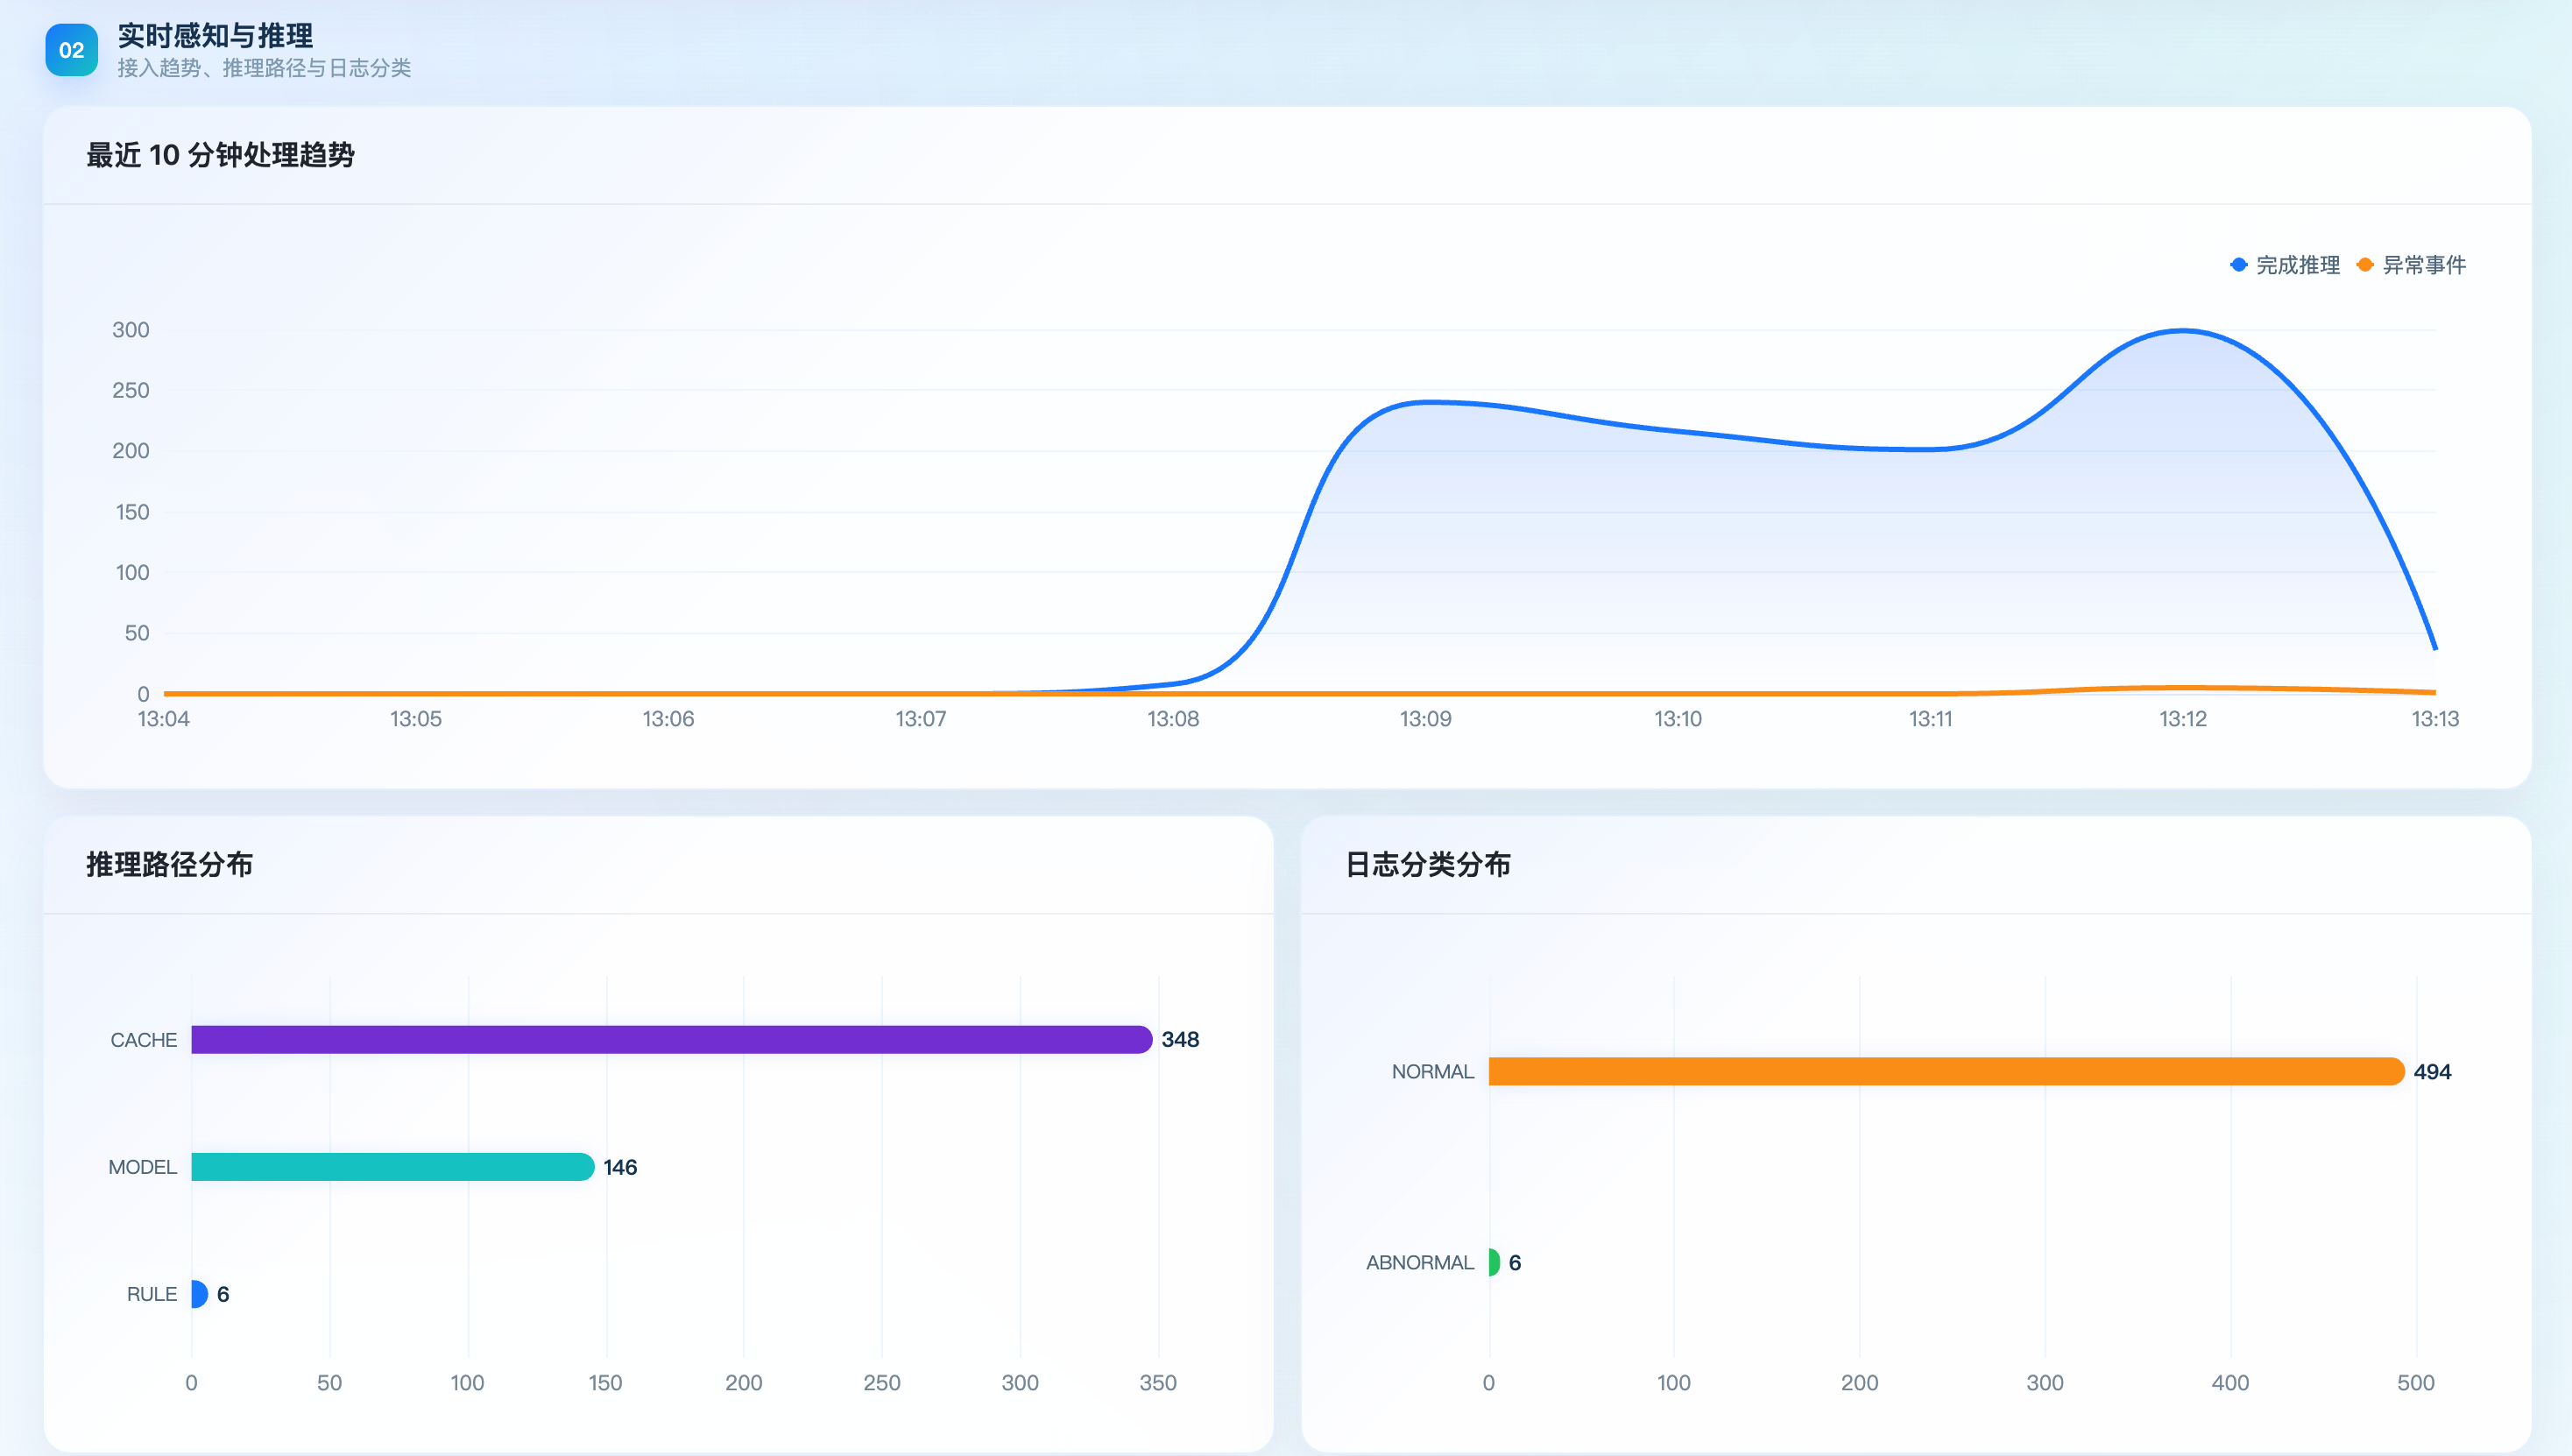
\includegraphics[width=0.98\textwidth]{figures/s-02c-inference-trend-and-distribution.png}
  \caption{当前运行窗口的处理趋势、推理路径与日志类别分布}
  \label{fig:inference-trend}
\end{figure}

\cref{fig:inference-trend}把最近十分钟的处理趋势与 \texttt{CACHE/MODEL/RULE} 路径分布放在同一观察面中。它能够直观说明分层推理在运行时确实存在不同早停路径，并帮助运维人员发现异常比例或某类推理路径的突变。图中数量属于截图对应的运行窗口，不用于推导长期业务比例。

\begin{figure}[htbp]
  \centering
  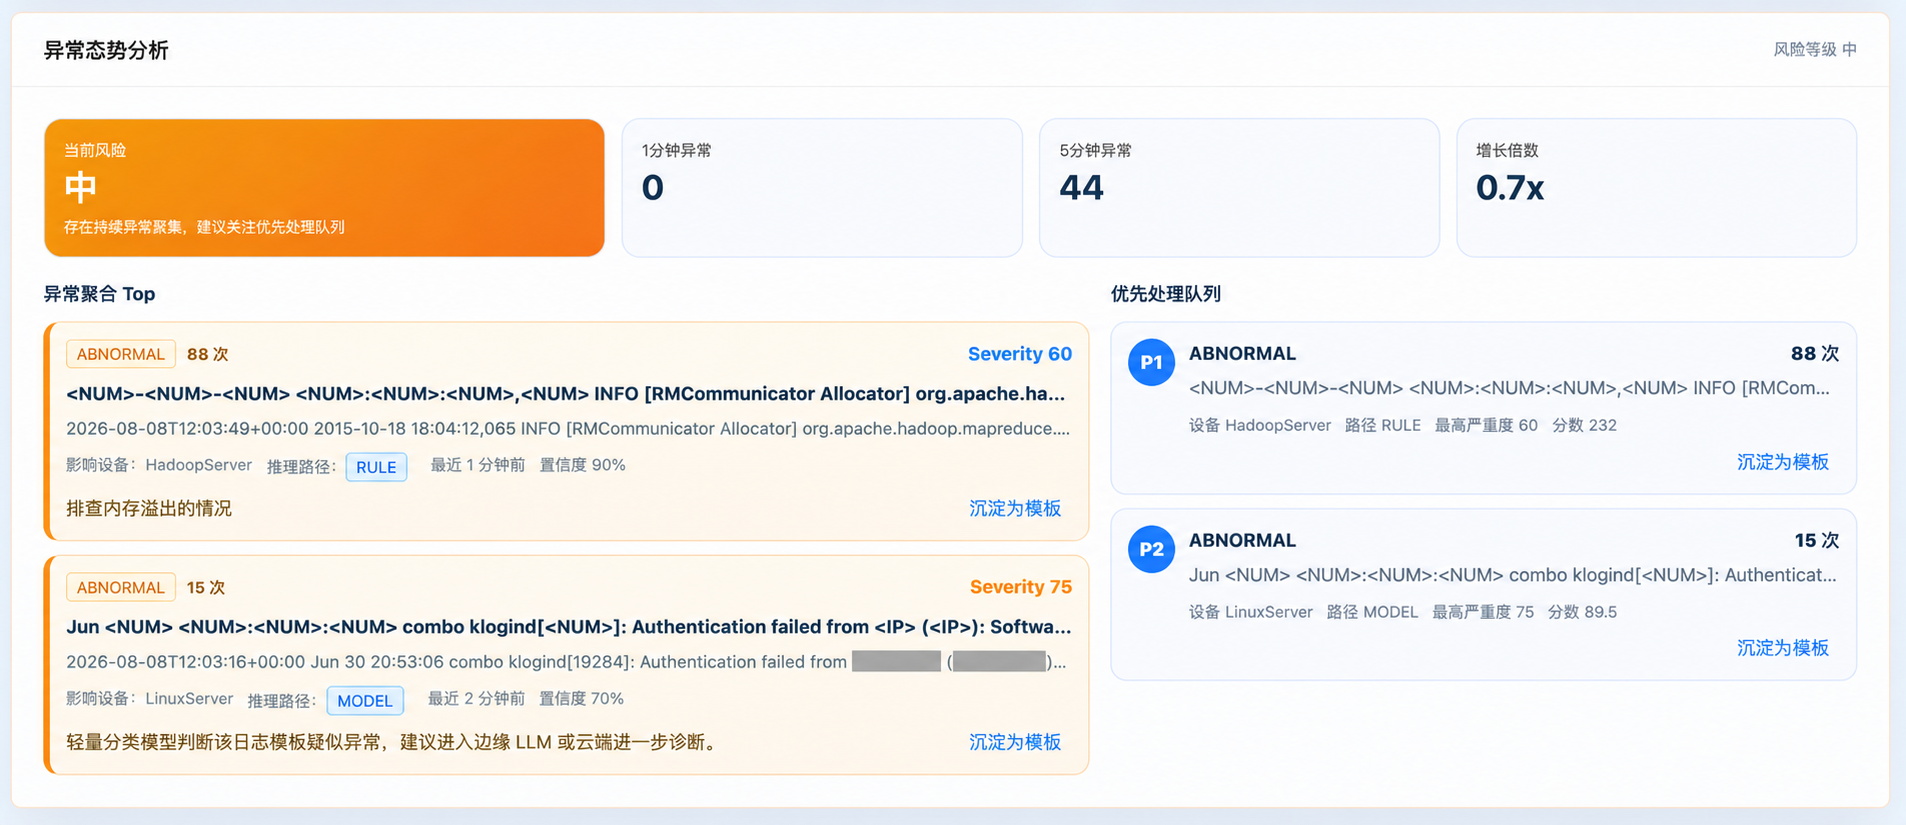
\includegraphics[width=0.98\textwidth]{figures/s-03-anomaly-trend-analysis-redacted.png}
  \caption{历史日志回放中的异常聚合与优先处理队列}
  \label{fig:anomaly-analysis}
\end{figure}

\cref{fig:anomaly-analysis}展示了异常模板聚合、风险等级和优先处理队列。该页面基于脱敏后的历史日志样本回放，用于说明系统如何把分散事件组织成运维可读的异常态势，不将其描述为真实生产事故。

\section{规则与模型在线治理}
规则、模板和模型配置由 Server 发布，\texttt{edge-infer} 使用 ETag 轮询。完整响应会先完成解析与校验；校验失败时继续使用上一份有效配置，校验通过后再更新知识和模型子系统。ETag 相当于配置内容的版本指纹：内容未变化时不重复传输，内容变化时才触发更新。

\begin{figure}[htbp]
  \centering
  \begin{subfigure}[t]{0.49\textwidth}
    \centering
    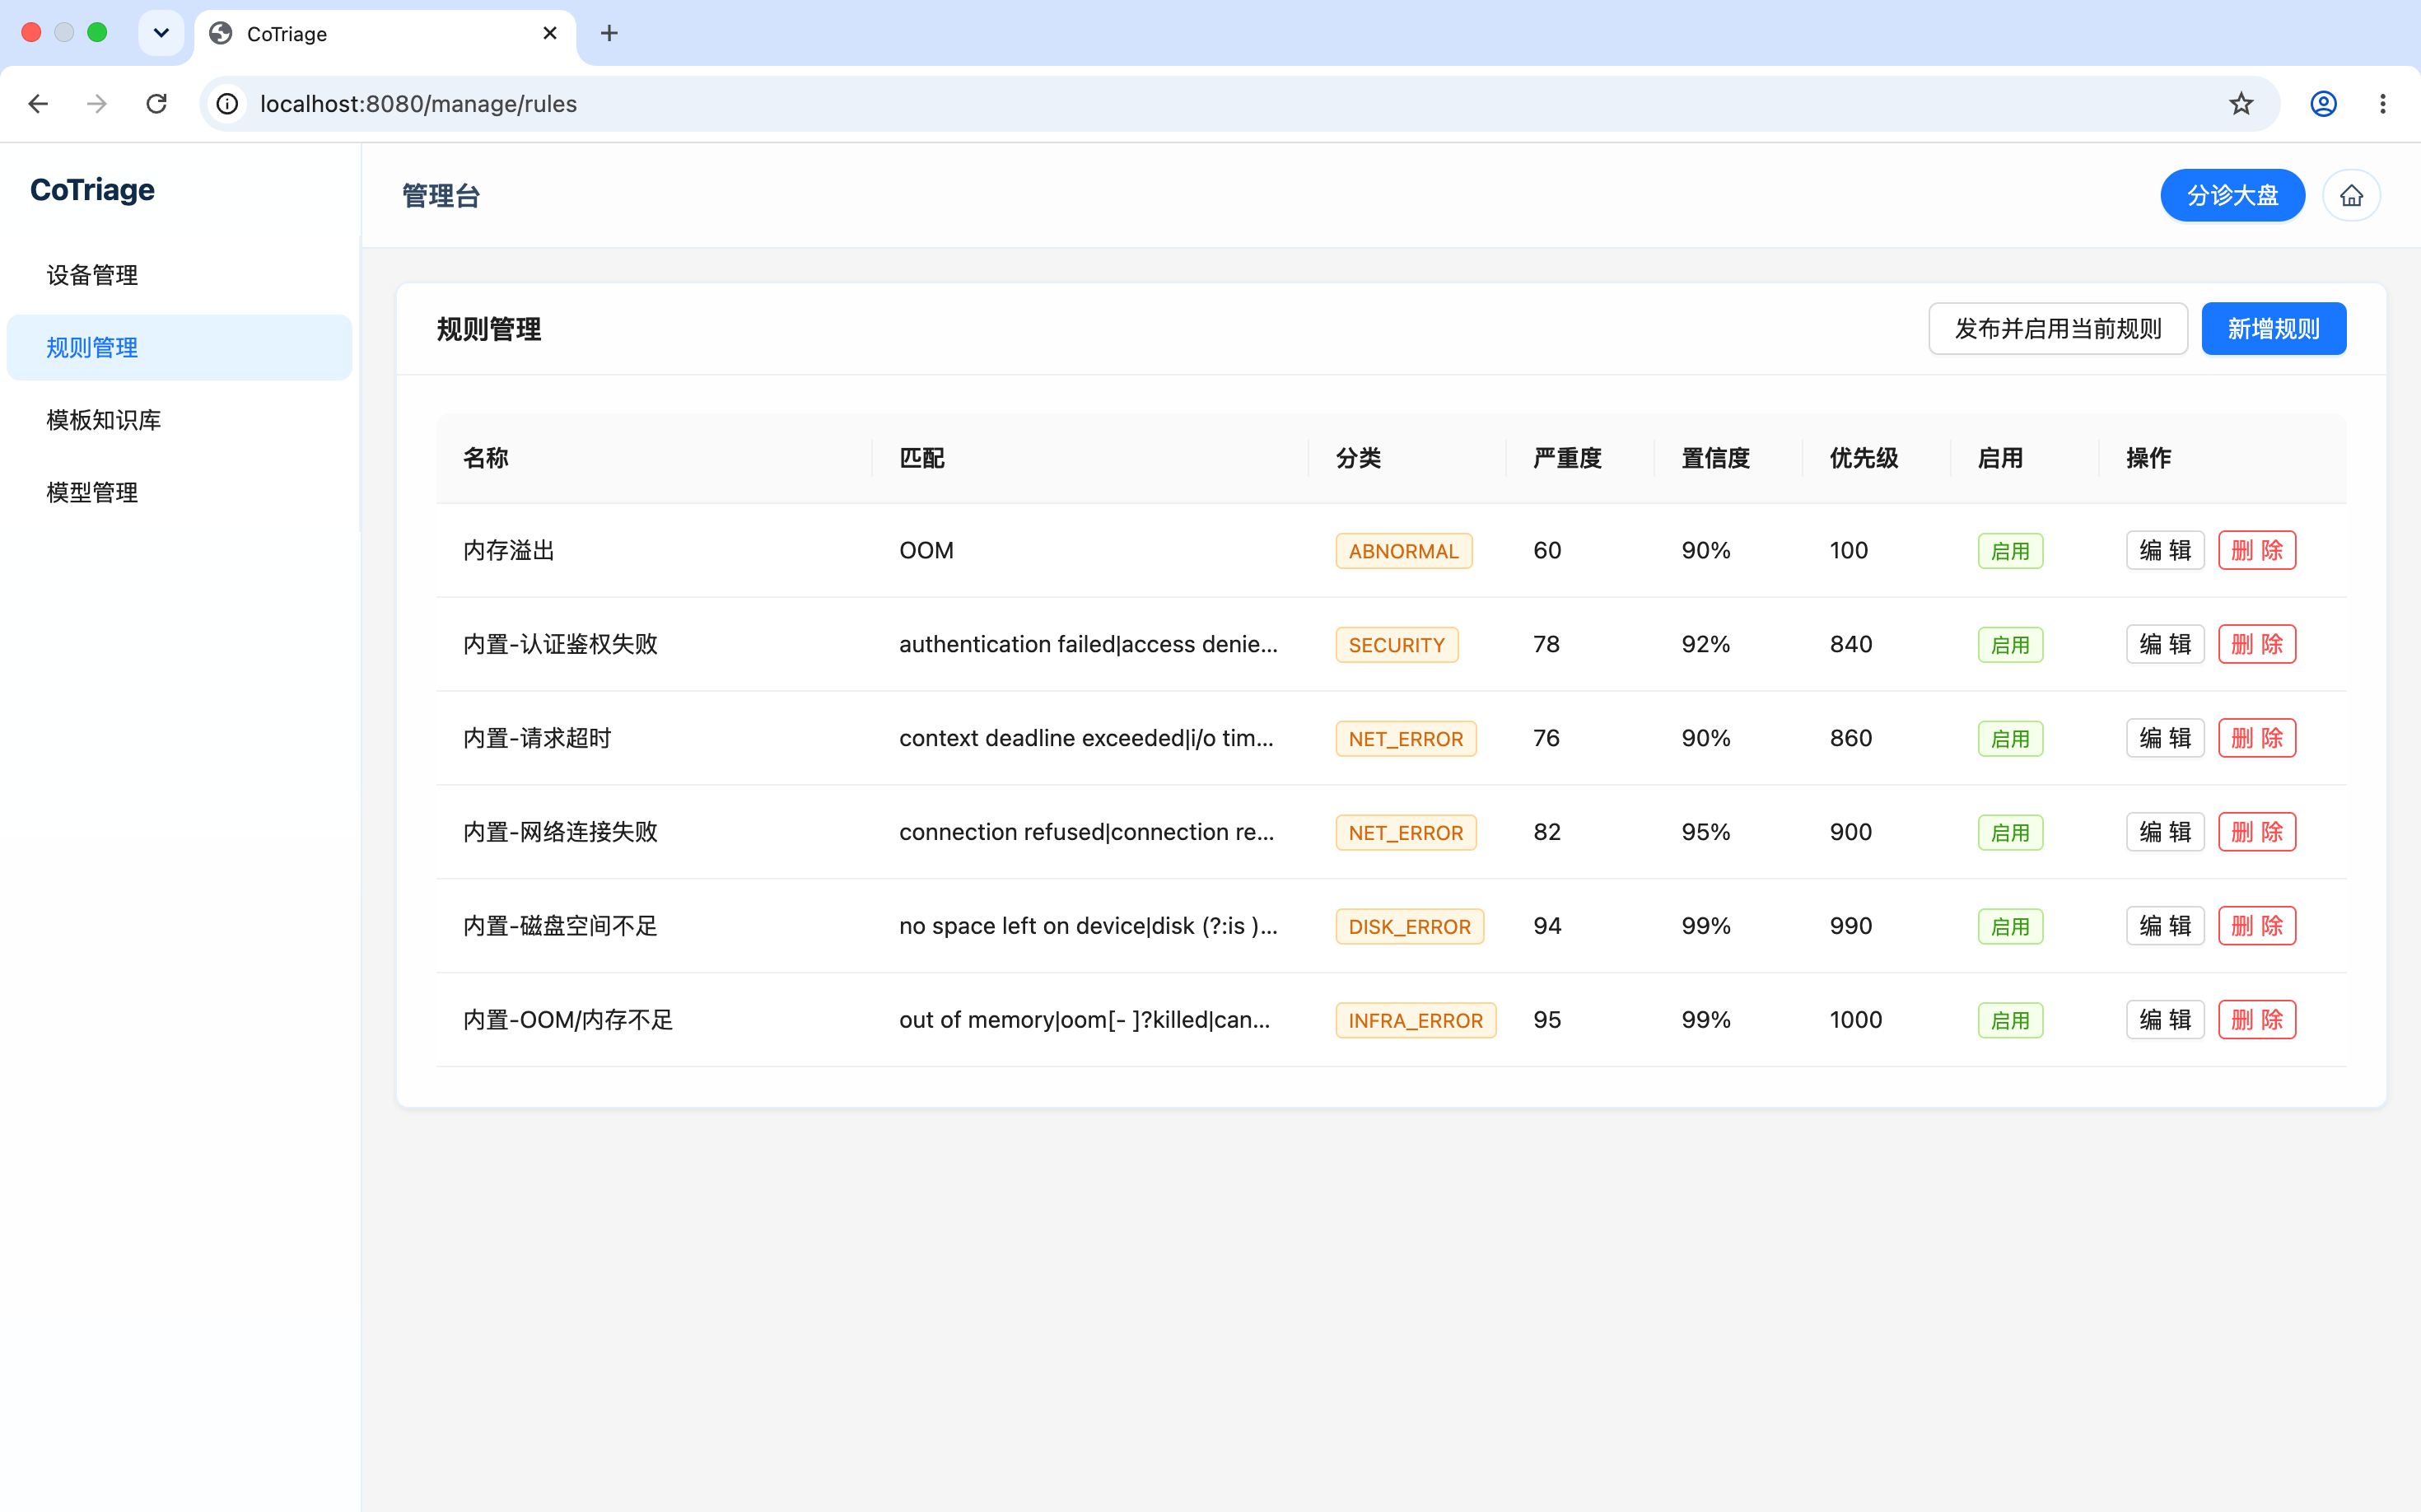
\includegraphics[width=\linewidth]{figures/s-08a-rule-management.png}
    \caption{规则发布与启用}
  \end{subfigure}\hfill
  \begin{subfigure}[t]{0.49\textwidth}
    \centering
    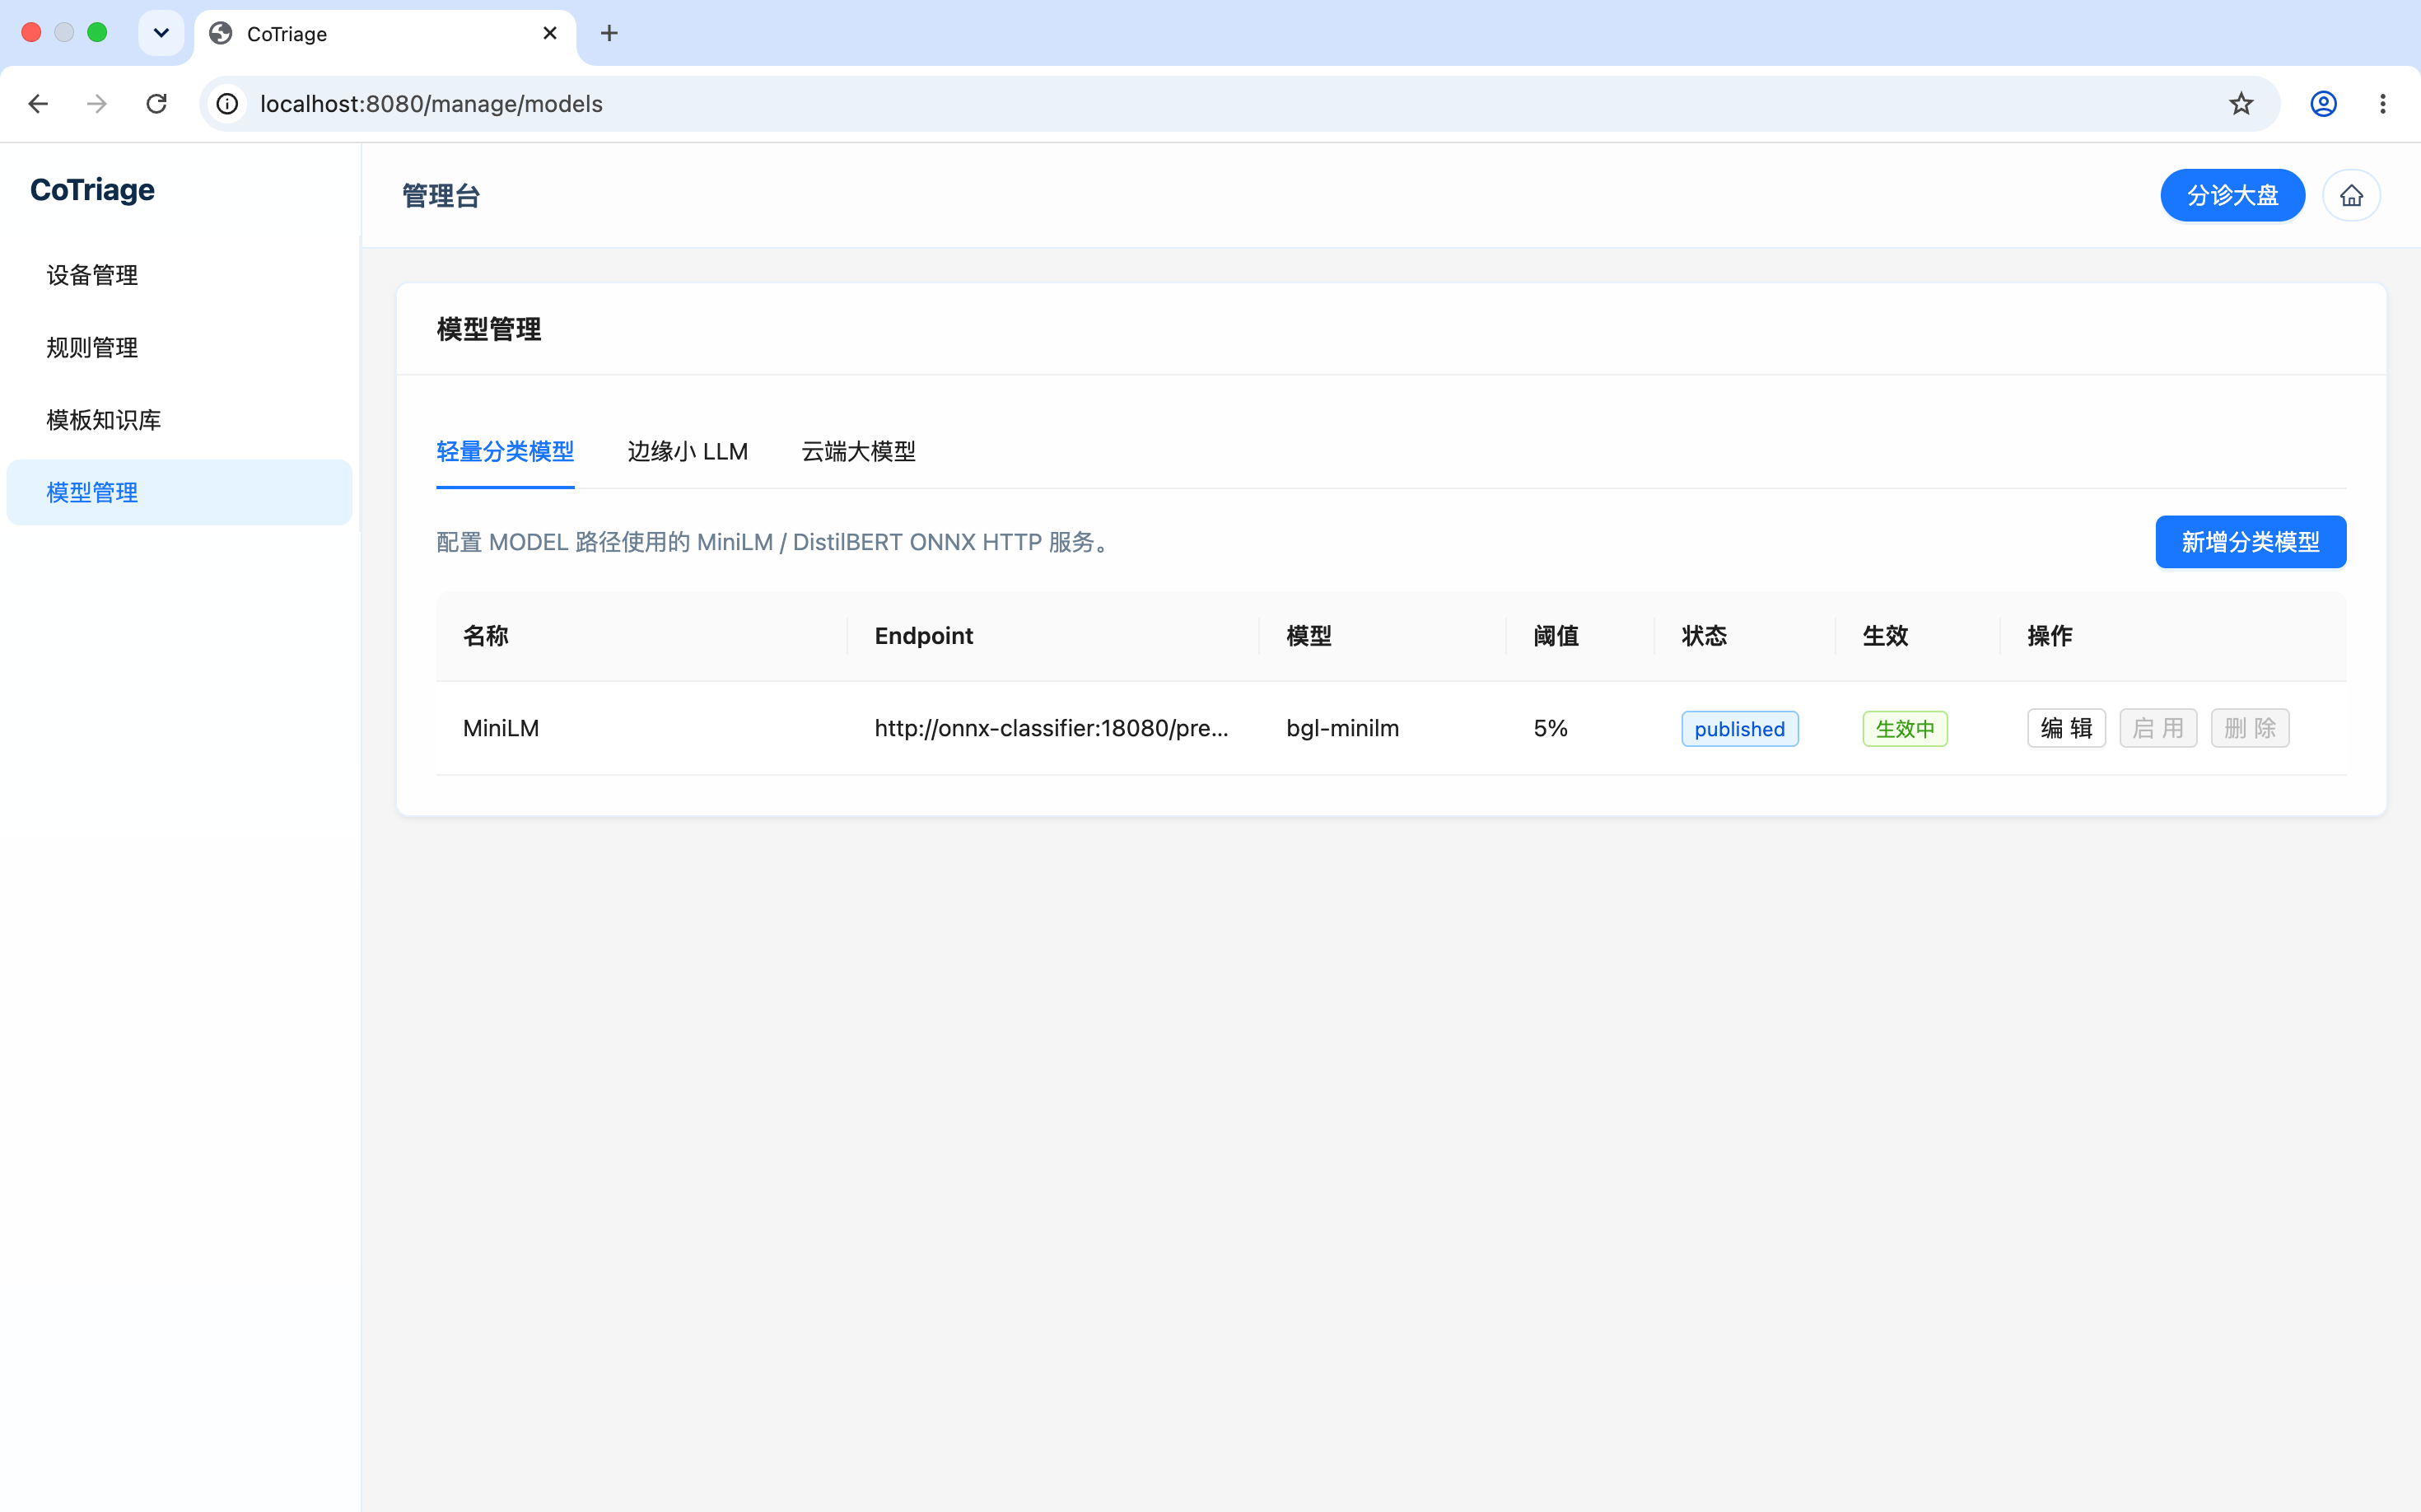
\includegraphics[width=\linewidth]{figures/s-09a-minilm-model-management.png}
    \caption{MiniLM 模型发布与生效}
  \end{subfigure}
  \caption{边缘知识与模型的在线配置入口}
  \label{fig:edge-config}
\end{figure}

\cref{fig:edge-config}说明规则和轻量模型可以通过统一管理台发布并查看生效状态。配置版本与事件结果共同保存，使运维人员能够回答“当时使用了哪一份规则或模型”，也为回滚和问题定位提供基础。
